%	Name			:: 	sthlm Beamer Theme  HEAVILY based on the hsrmbeamer theme (Benjamin Weiss)
%	Author			:: 	Mark Hendry Olson (mark@hendryolson.com)
%	Created			::	2013-07-31
%	Updated	    	::	[[April]] 04, 2017 at 16:26:39
%	Version			:: 	2.0.2
%	Email			:: 	hendryolson@gmail.com
%	Website			:: 	http://markolson.se
%	Twitter			:: 	markolsonse
%	Instagram		:: 	markolsonse
%
%	License			:: 	This file may be distributed and/or modified under the
%					GNU Public License.
%
%	Description		::	This presentation is a demonstration of the sthlm beamer
%					theme, which is HEAVILY based on the HSRM beamer theme created by Benjamin Weiss
%					(benjamin.weiss@student.hs-rm.de), which can be found on GitHub
%					<https://github.com/hsrmbeamertheme/hsrmbeamertheme>.  It also borrows heavily
%					from the work of Matthias Vogelgesang, (https://bloerg.net) and his Metropolis Mtheme,
%					<https://github.com/matze/mtheme>.
%
%	Theme			::	newPxFont
%	Options			::	progressbar
%					::	sectionpages
%					::	numfooter
%					::	fullfooter
%					::	dovaligncolumns
%					::	protectframetitle
%					::	greybg
%					::	cblock
%					::	minimal
%					::  displaynote


%-=-=-=-=-=-=-=-=-=-=-=-=-=-=-=-=-=-=-=-=-=-=-=-=
%
%        LOADING DOCUMENT
%
%-=-=-=-=-=-=-=-=-=-=-=-=-=-=-=-=-=-=-=-=-=-=-=-=

\documentclass[newPxFont, fullfooter, sectionpages, progressbar]{beamer}
\usepackage[utf8]{inputenc}
%\usepackage{xeCJK}
\usetheme{sthlm}
\usepackage{pgfplots}
\pgfplotsset{compat=1.14}
\usepackage{cancel}
\usepackage{graphicx} %use graph format
\usepackage{epstopdf}
\usepackage{ragged2e}
\usepackage{hyperref}
\usepackage[labelformat=empty]{caption}



%-=-=-=-=-=-=-=-=-=-=-=-=-=-=-=-=-=-=-=-=-=-=-=-=
%
%	PRESENTATION INFORMATION
%
%-=-=-=-=-=-=-=-=-=-=-=-=-=-=-=-=-=-=-=-=-=-=-=-=
% \useoutertheme[subsection=false]{miniframes}		% display outline in the top

\title{\centering Bottle Detection in the Wild Using Low-Altitude Unmanned Aerial Vehicles}
% \subtitle{}

\author{\small Jinwang Wang \and Wei Guo \and Ting Pan \and Huai Yu \and Lin Duan \and \underline{\textbf{Wen Yang}}}
\institute{Wuhan University, Wuhan, China}
\date{2018.07.10-2018.07.13 Fusion 2018}
\hypersetup{pdfauthor = {jwwangchn: jwwangchn@outlook.com},
pdfsubject = {Beamer},
pdfkeywords = {Beamer theme, sthlm},
pdfmoddate= {D:\pdfdate},
pdfcreator = {}
}

\begin{document}

%-=-=-=-=-=-=-=-=-=-=-=-=-=-=-=-=-=-=-=-=-=-=-=-=
%
%	TITLE PAGE
%
%-=-=-=-=-=-=-=-=-=-=-=-=-=-=-=-=-=-=-=-=-=-=-=-=

\maketitle
\note{Good afternoon, everyone. I am Jinwang Wang from Wuhan University. In the next few minutes, I will introduce our ``Bottle Detection in the Wild Using Low-Altitude Unmanned Aerial Vehicles''.}


%-=-=-=-=-=-=-=-=-=-=-=-=-=-=-=-=-=-=-=-=-=-=-=-=
%
%	TABLE OF CONTENTS: OVERVIEW
%
%-=-=-=-=-=-=-=-=-=-=-=-=-=-=-=-=-=-=-=-=-=-=-=-=

\section*{Outline}
\begin{frame}{Outline}
% For longer presentations use hideallsubsections option
\tableofcontents[hideallsubsections]
\note{I will talk my work through the following sections.}
\end{frame}

%-=-=-=-=-=-=-=-=-=-=-=-=-=-=-=-=-=-=-=-=-=-=-=-=
%
%	TABLE OF CONTENTS: OVERVIEW
%
%-=-=-=-=-=-=-=-=-=-=-=-=-=-=-=-=-=-=-=-=-=-=-=-=

\section{Introduction}
\note{First, introduction.}
%-=-=-=-=-=-=-=-=-=-=-=-=-=-=-=-=-=-=-=-=-=-=-=-=
%	FRAME: Motivation
%-=-=-=-=-=-=-=-=-=-=-=-=-=-=-=-=-=-=-=-=-=-=-=-=

\begin{frame}[c]{Motivation}
	It's very \cBlue{dangerous} for the sanitation workers who pick up rubbish on the mountain. Can we help them? Yes!
	\begin{figure}
		\centering
		\only<1>
		{
			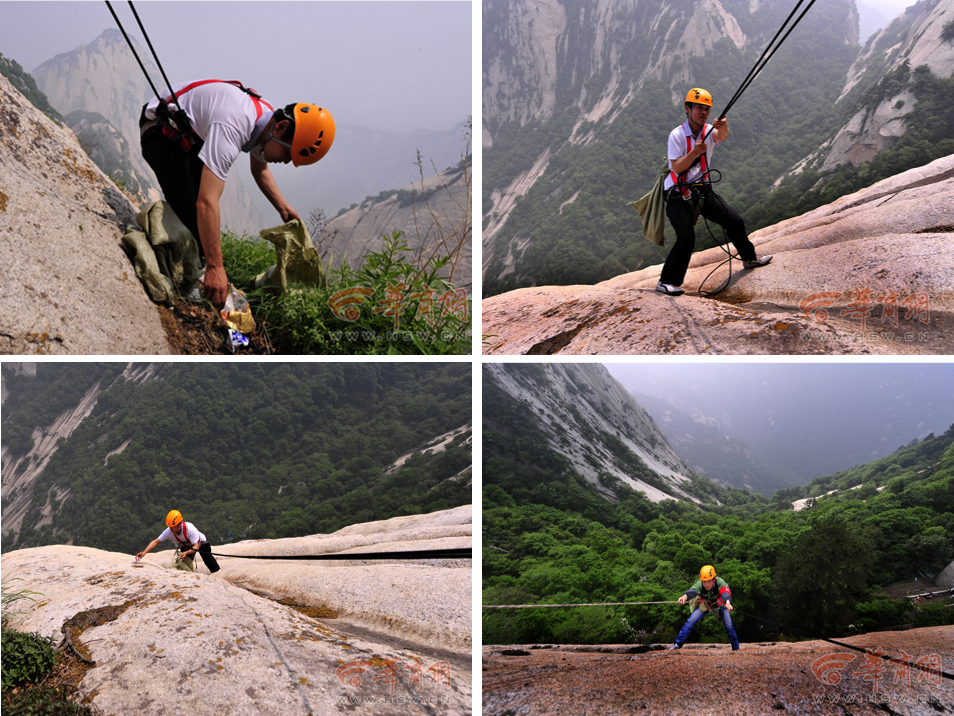
\includegraphics[height=0.5\textheight]{images/sanitation_worker.png}
			\caption*{The sanitation workers on the Huashan Mountain.}
		}
		\only<2>{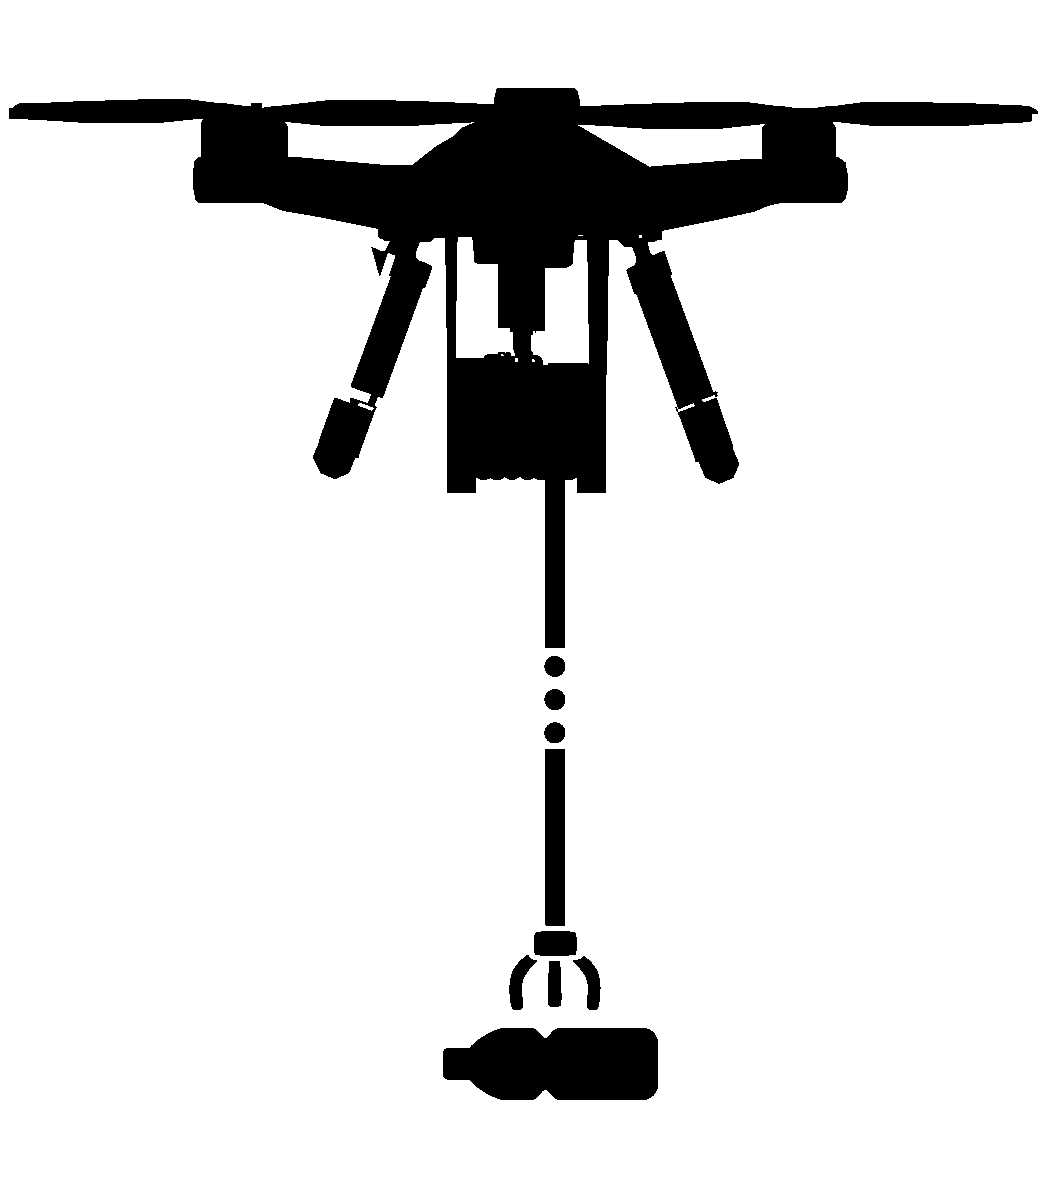
\includegraphics[height=0.6\textheight]{images/illustrater.pdf}}
	\end{figure}
	\begin{center}
		\only<2>{\large{\cBlue{UAVs can help them!}}}
	\end{center}

	\note{As well we know, It's very \cBlue{dangerous} for the sanitation workers who pick up rubbish on the mountain. So can we help them? Yes! We can use UAV to pick bottles.}
\end{frame}

%-=-=-=-=-=-=-=-=-=-=-=-=-=-=-=-=-=-=-=-=-=-=-=-=
%	FRAME: Pipeline
%-=-=-=-=-=-=-=-=-=-=-=-=-=-=-=-=-=-=-=-=-=-=-=-=

\begin{frame}[c]{Pipeline}
	\begin{figure}
		\centering
		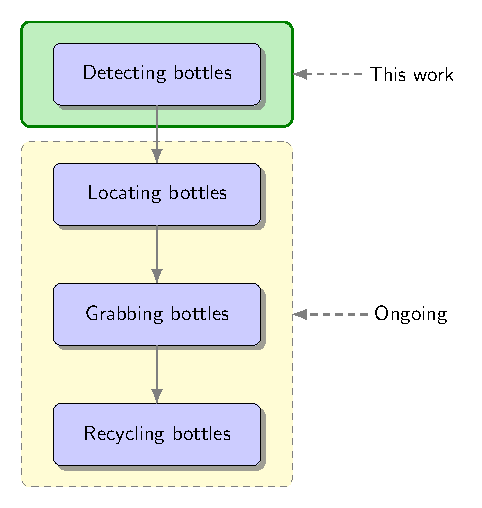
\includegraphics[height=0.85\textheight]{images/pipeline.pdf}
	\end{figure}
	\note{This work mainly focuses on bottles detection. The whole pipeline is shown as below. After bottles detection, bottles location, grab bottles and recycle is going on.}
\end{frame}

%-=-=-=-=-=-=-=-=-=-=-=-=-=-=-=-=-=-=-=-=-=-=-=-=
%	FRAME: Bottles in Different Dataset
%-=-=-=-=-=-=-=-=-=-=-=-=-=-=-=-=-=-=-=-=-=-=-=-=

\begin{frame}[c]{challenges}
	\only<1-2>{\justifying{In UAV images, the bottles look completely different from the bottles in datasets such as PASCAL VOC, Microsoft COCO, etc.}}
	\only<3->{\justifying{As to UAV images, detecting bottles exists several unique challenges.}}
	\begin{figure}
		\centering
		\only<1-2>{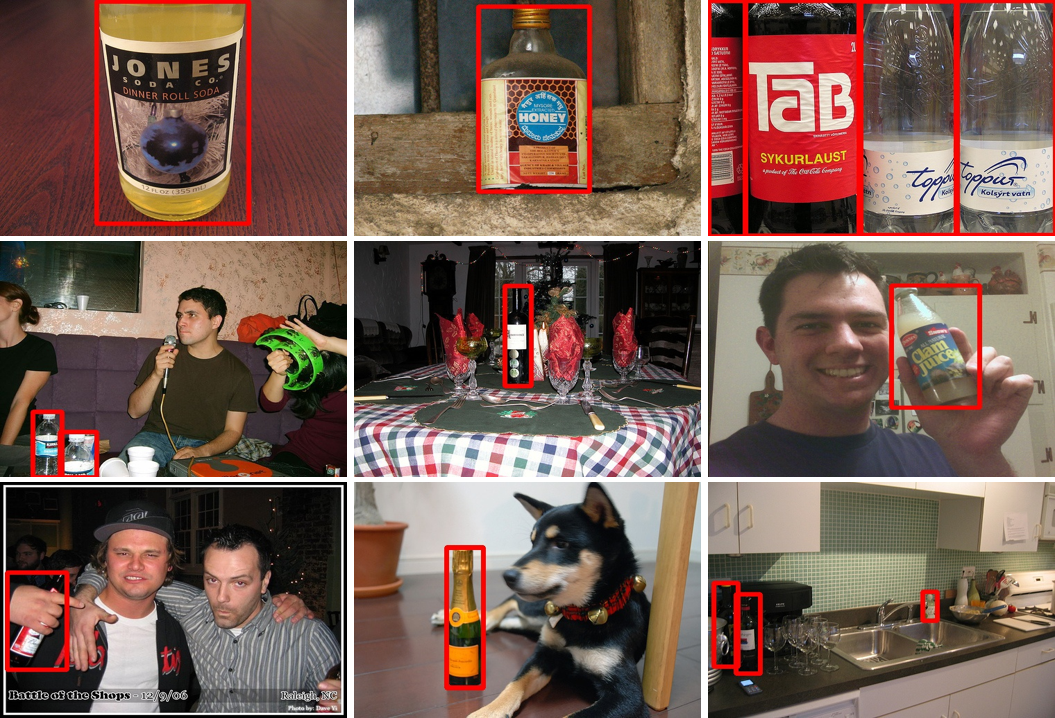
\includegraphics[height=0.5\textheight]{images/bottle_VOC.png}
		\hspace{0.1cm}}
		\only<2>{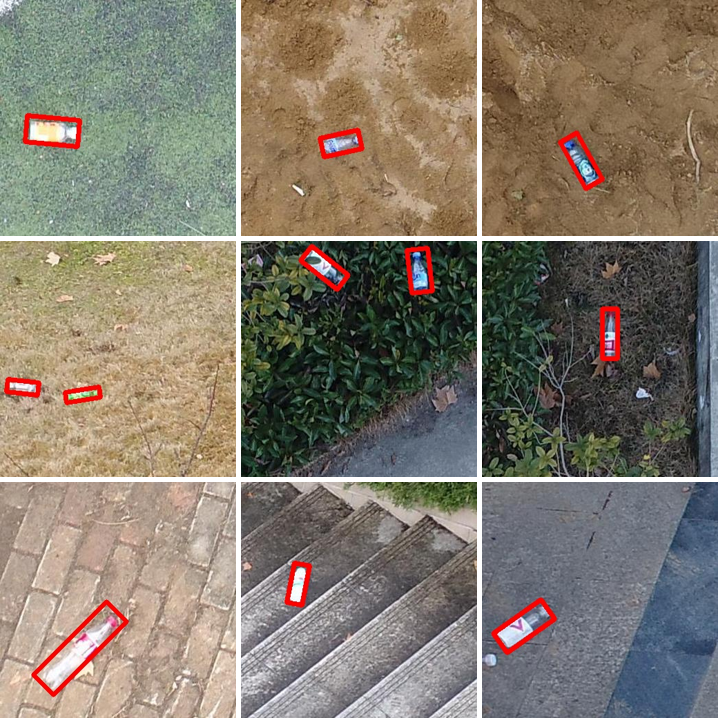
\includegraphics[height=0.5\textheight]{images/bottle_UAV.png}}
	\end{figure}
	
	\only<3->
	{
		\begin{columns}
			\begin{column}{0.4\linewidth}
				\centering
				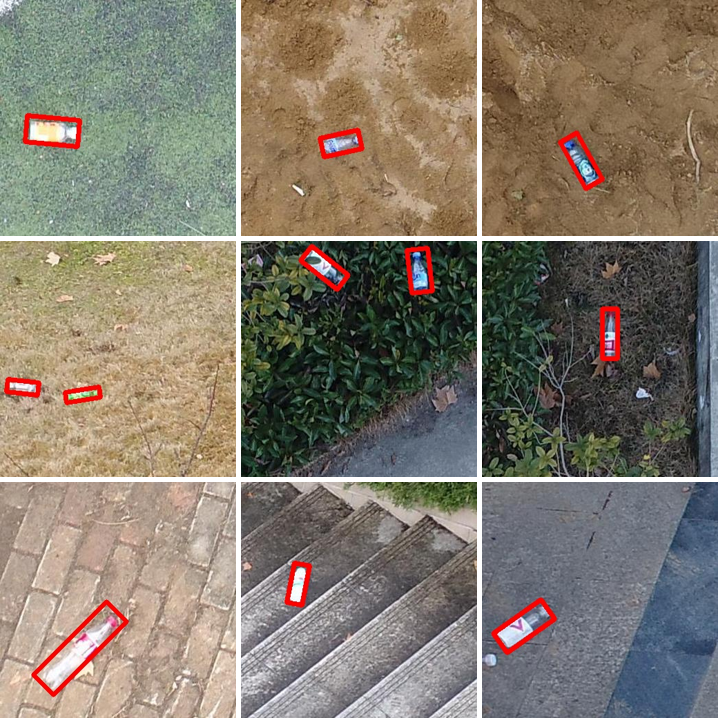
\includegraphics[width=0.9\textwidth]{images/bottle_UAV.png}
			\end{column}
	
			\begin{column}{0.6\linewidth}
				\begin{itemize}
					\item<3-> \footnotesize{The size is very small, generally less than $50\times 50$ pixels.}
					\item<4-> \footnotesize{Backgrounds are very complex.}
					\item<5-> \footnotesize{Arbitrary orientations.}
					\item<6-> \footnotesize{Plastic bottles are often transport, increaseing the difficulty of detection.}
				\end{itemize}
			\end{column}
		\end{columns}
		\vspace{1cm}
	}
	
	
	\only<1>{\note{In order to detect bottles on UAV, a high quality bottle dataset is needed for training deep learning based detection models. There are exactly bottles in the PASCAL VOC, Microsoft COCO, etc. datasets, why don't we use these bottles to training models?}}

	\only<2>{\note{Because in UAV images, the bottles look completely different from the bottles in PASCAL VOC etc. datasets. As to UAV image, as you can see, detecting bottles exists several unique challenges. First, bottles are very small, generally less than $50\times 50$ pixels; Second, the backgrounds of the bottles are very complex. Third, in contrast to conventional object detection dataset, the bottles in UAV images often appear with arbitrary orientations. Fourth, plastic bottles are often transparent, thus the background will can be seen through the bottles.}}
\end{frame}

%-=-=-=-=-=-=-=-=-=-=-=-=-=-=-=-=-=-=-=-=-=-=-=-=
%
%	SECTION: COLORS
%
%-=-=-=-=-=-=-=-=-=-=-=-=-=-=-=-=-=-=-=-=-=-=-=-=
\section{UAV-Bottle Dataset}

%-=-=-=-=-=-=-=-=-=-=-=-=-=-=-=-=-=-=-=-=-=-=-=-=
%	FRAME: Dataset
%-=-=-=-=-=-=-=-=-=-=-=-=-=-=-=-=-=-=-=-=-=-=-=-=
\begin{frame}{Dataset}
	\justifying{To build a baseline for bottle detection in UAV images, we establish a large scale bottle detection dataset, we call \cBlue{UAV-Bottle Dataset(UAV-BD)} and benchmark.}

	\note{To build a baseline for bottle detection in UAV images, we establish a large scale bottle detection dataset, we call \cBlue{UAV-Bottle Dataset(UAV-BD)} and benchmark.}
\end{frame}

%-=-=-=-=-=-=-=-=-=-=-=-=-=-=-=-=-=-=-=-=-=-=-=-=
%	FRAME: Dataset Collection
%-=-=-=-=-=-=-=-=-=-=-=-=-=-=-=-=-=-=-=-=-=-=-=-=
\begin{frame}{Dataset Collection}
	\justifying{We used \cBlue{DJI Phantom 4 Pro} to collect images. The resolution of the captured images are \cBlue{$5472 \times 3078$ pixels}. At the same time, we follow four key suggestions:}
	\vspace{0.4cm}
	\begin{columns}
		\begin{column}{0.48\linewidth}
			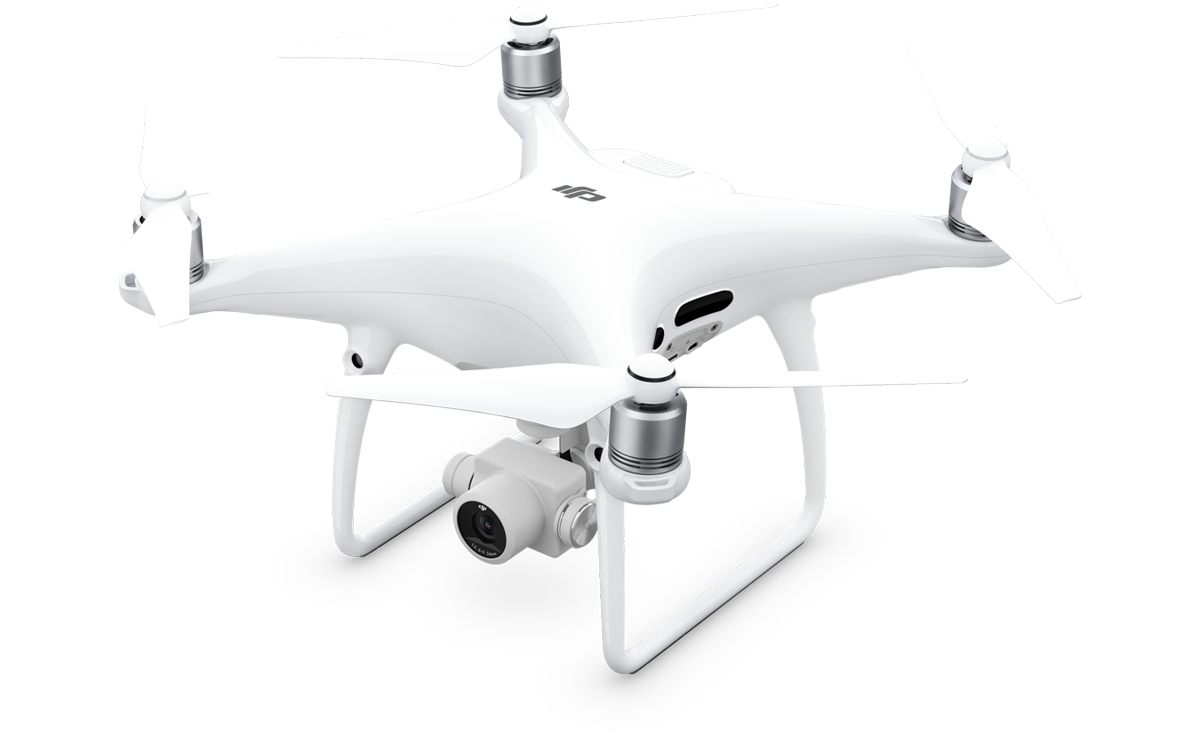
\includegraphics[width=\textwidth]{images/DJI_Phantom4.png}
		\end{column}

		\begin{column}{0.48\linewidth}
			\begin{itemize}
				\item<1-> \small{Wide range of scale and aspect ratios.}
				\item<2-> \small{Different backgrounds.}
				\item<3-> \small{Different orientation.}
				\item<4-> \small{As many types of bottles as possible.}
			\end{itemize}
		\end{column}
	\end{columns}

	\note{We use DJI Phantom 4 Pro to collect images. The resolution of the captured images are \cBlue{$5472 \times 3078$ pixels}. At the same time, we follow four key suggestions. First, collecting images including bottles a wide range of scale and aspect ratio. Second, collecting images including different backgrounds. Third, collecting images including bottles different orientations. Third, collecting as many types of bottles as possible.}
\end{frame}

%-=-=-=-=-=-=-=-=-=-=-=-=-=-=-=-=-=-=-=-=-=-=-=-=
%	FRAME: Dataset Collection
%-=-=-=-=-=-=-=-=-=-=-=-=-=-=-=-=-=-=-=-=-=-=-=-=

\begin{frame}{Dataset Collection}

	\cBlue{8 background scenes} are chosen and annotated in our UAV-BD:

	\begin{columns}[c]
		\begin{column}{0.3\textwidth}
			\begin{itemize}
			\item \small{Bushforest land}
			\item \small{Waste land}
			\item \small{Step}
			\item \small{Forest land}
			\end{itemize}
		\end{column}

		\begin{column}{0.3\textwidth}
			\begin{itemize}
			\item \small{Flat land}
			\item \small{Plastic stadium}
			\item \small{Sand land}
			\item \small{Grassland}
			\end{itemize}
		\end{column}
	\end{columns}
	\begin{figure}
		\centering
		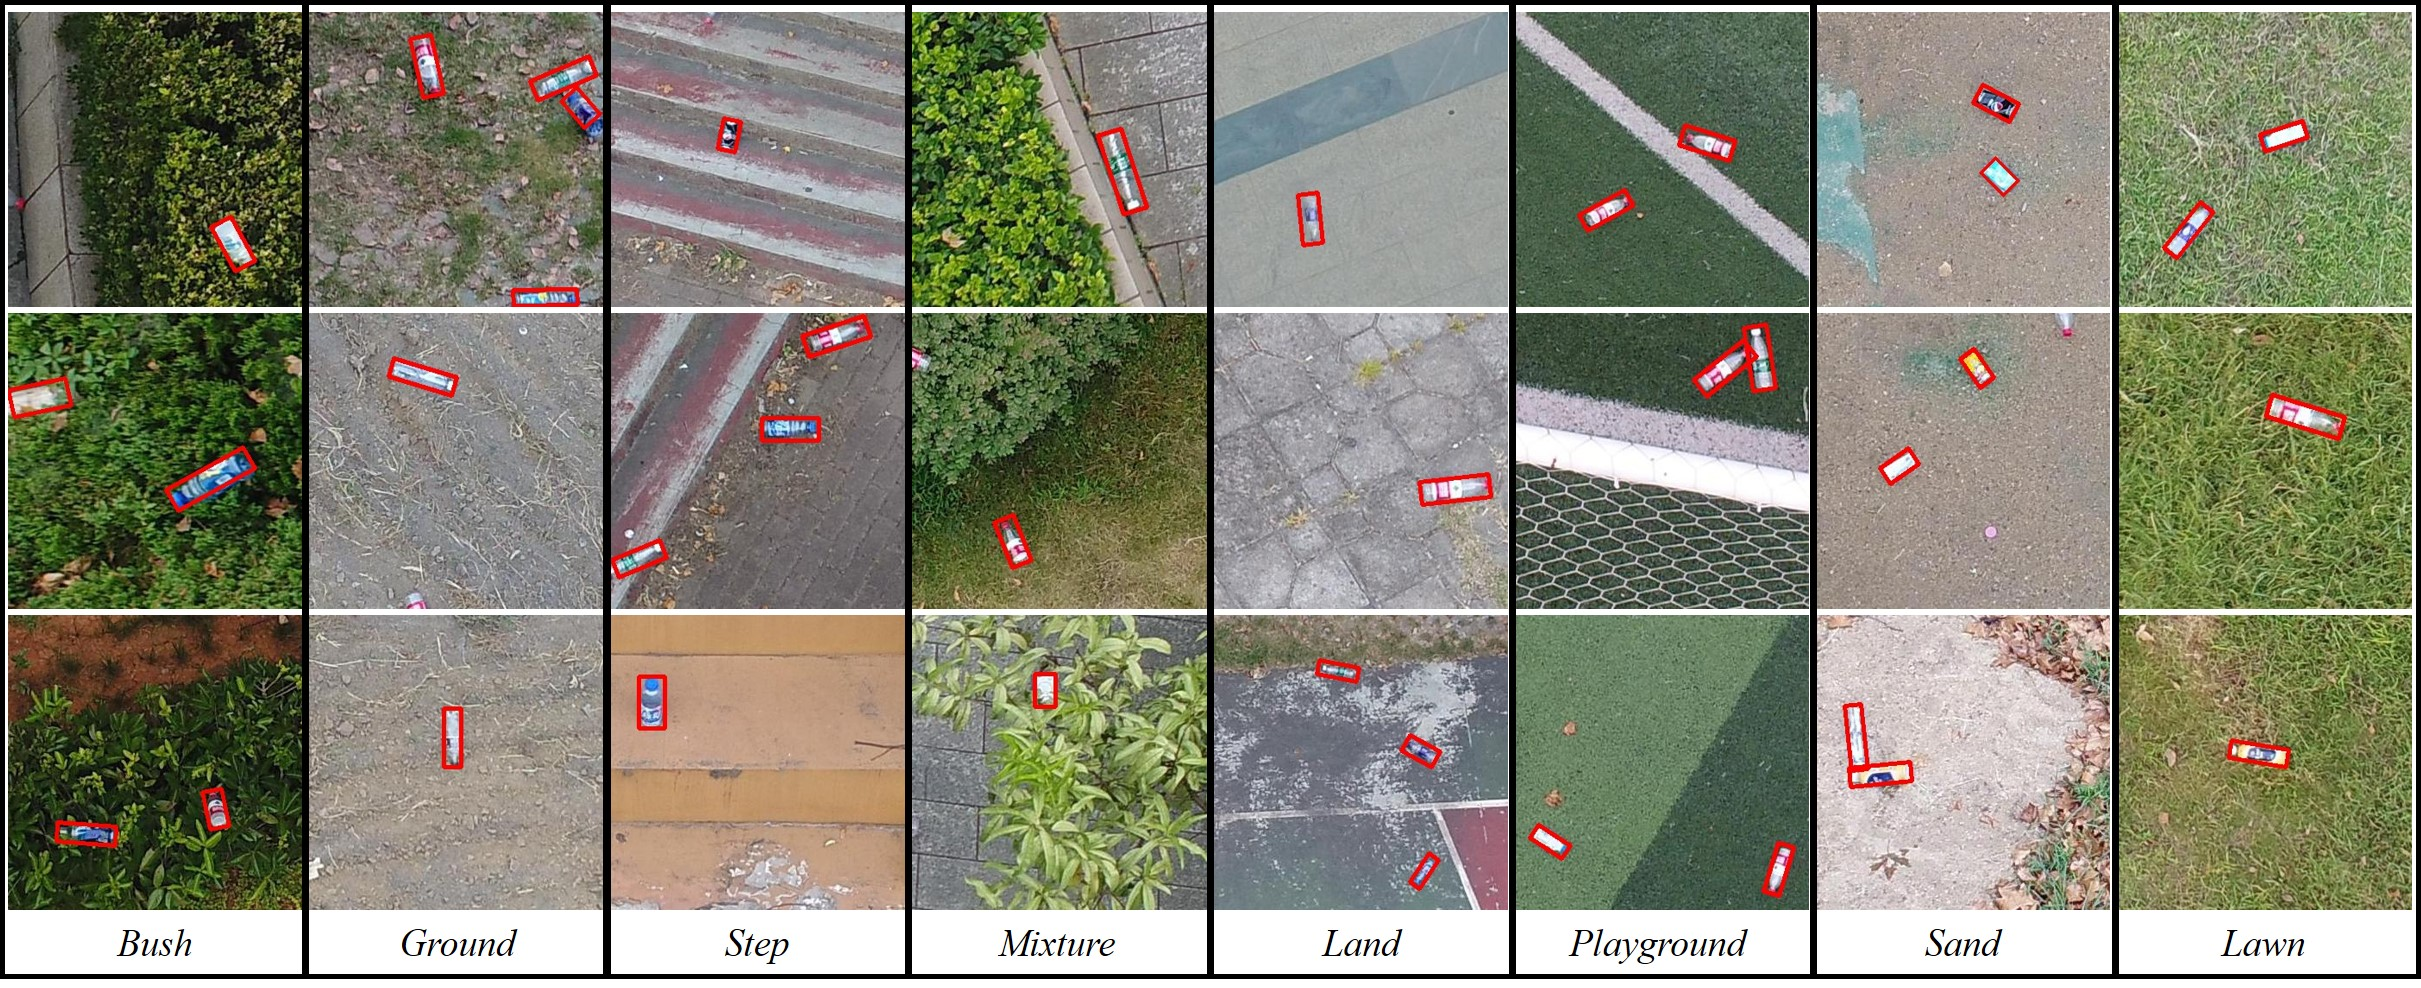
\includegraphics[width=0.9\textwidth]{images/dataset1.jpg}
	\end{figure}
	\note{Eight background scenes are chosen and annotated in our UAV-BD, including Bush forest land, Waste land, Step, Forest land, Flat land, Plastic stadium, Sand land, Grassland.}
\end{frame}

%-=-=-=-=-=-=-=-=-=-=-=-=-=-=-=-=-=-=-=-=-=-=-=-=
%	FRAME: Annotation Method
%-=-=-=-=-=-=-=-=-=-=-=-=-=-=-=-=-=-=-=-=-=-=-=-=

\begin{frame}{Annotation Method}
	\justifying{\footnotesize{A common description of horizontal bounding boxes is \cBlue{$(c_x, c_y, h, w)$} , where $(c_x, c_y)$ is the center location, $h$, $w$ are the height and width.}}
	\begin{figure}
		\centering
		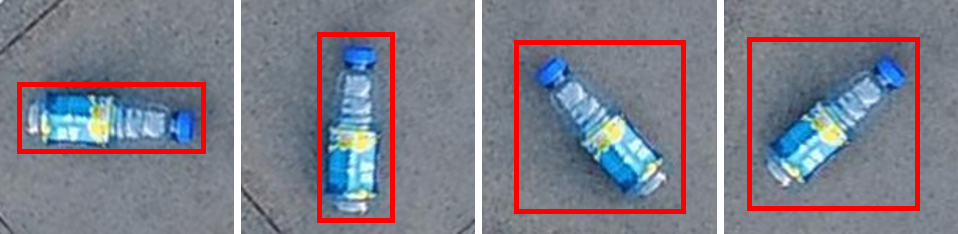
\includegraphics[width=0.6\textwidth]{images/HBB.png}
	\end{figure}
	\justifying{\footnotesize{However, horizontal bounding box cannot accurately or compactly outline oriented instances such as the bottles in UAV images. So we use  \cBlue{$(c_x, c_y, h, w, \theta)$} to describe bounding boxes, where $\theta$ is the angle from the horizontal direction of the horizontal bounding box.}}
	\begin{figure}
		\centering
		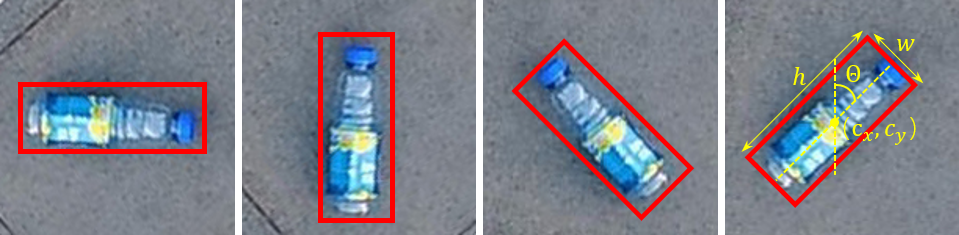
\includegraphics[width=0.6\textwidth]{images/OBB.png}
	\end{figure}
	\note{A common description of horizontal bounding boxes is \cBlue{$(c_x, c_y, h, w)$} , where $(c_x, c_y)$ is the center location, $h$, $w$ are the height and width. However, horizontal bounding box cannot accurately or compactly outline oriented instances such as the bottles in UAV images. So we use  \cBlue{$(c_x, c_y, h, w, \theta)$} to describe bounding boxes, where $\theta$ is the angle from the horizontal direction of the horizontal bounding box.}
\end{frame}

%-=-=-=-=-=-=-=-=-=-=-=-=-=-=-=-=-=-=-=-=-=-=-=-=
%	Dataset Statistics
%-=-=-=-=-=-=-=-=-=-=-=-=-=-=-=-=-=-=-=-=-=-=-=-=

\begin{frame}{Dataset Statistics}
	\justifying{\footnotesize{The size of original image(OI) in UAV-BD is \cBlue{$5472\times 3078$ pixels}, they are too large to be trained for CNN-based algorithms. So we segment each OI into $144$ small subimages(SIs), and the size of SIs is \cBlue{$342\times 342$ pixels}. Images and instances number in UAV-BD are shown in the table below.}}
	\begin{table}
		\centering
		\footnotesize
		% \caption{\footnotesize{Images and instances number in UAV-BD.}}
		\label{statistics}
		\begin{tabular}{@{}ccc|cc@{}}
			\toprule
			\textbf{Scenes}     & \textbf{OI} & \textbf{SI} & \textbf{Instances in OI} &\textbf{Instances in SI}  \\ \midrule
			\cBlue{Bushforest land}       & 230  & 4134  & 1812  & 3047  \\
			\cBlue{Wasteland}     & 379  & 7598  & 4355  & 5800  \\
			\cBlue{Step}       & 135  & 2691  & 1325  & 2106  \\
			\cBlue{Forest land}    & 285  & 5724  & 3702  & 4891  \\
			\cBlue{Flat land}       & 134  & 2803  & 1538  & 2142  \\
			\cBlue{Plastic stadium} & 336  & 6807  & 4180  & 4998  \\
			\cBlue{Sand land}       & 249  & 5570  & 2704  & 4008  \\
			\cBlue{Grassland}       & 456  & 9029  & 5778  & 7787  \\ \midrule
			\textbf{Total}      & 2204 & 44356 & 25394 & 34779 \\ \bottomrule
		\end{tabular}
	\end{table}
	\note{In our dataset, the size of original image is \cBlue{$5472\times 3078$ pixels}, they are too large to be trained for CNN-based algorithms. So we segment each original image into $144$ small subimages, and the size of subimages is \cBlue{$342\times 342$ pixels}. Images and instances number in UAV-BD are shown in the table below.}
\end{frame}

%-=-=-=-=-=-=-=-=-=-=-=-=-=-=-=-=-=-=-=-=-=-=-=-=
%	Dataset Statistics
%-=-=-=-=-=-=-=-=-=-=-=-=-=-=-=-=-=-=-=-=-=-=-=-=
\begin{frame}{Dataset Statistics}

	\begin{columns}
		\begin{column}{.48\linewidth}
			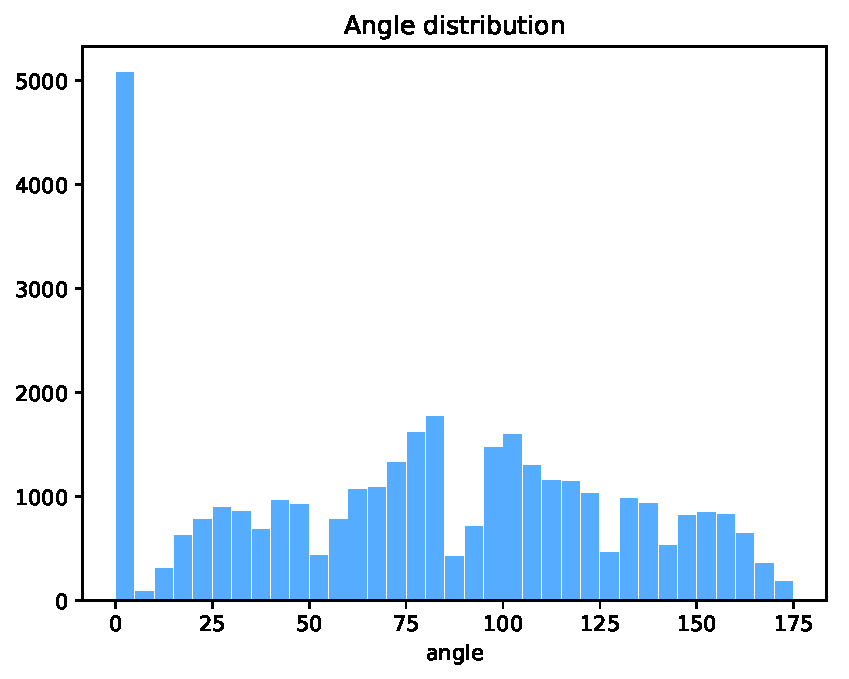
\includegraphics[width=\textwidth]{images/angle_hist.pdf}
		\end{column}

		\begin{column}{.48\linewidth}
			\justifying{\cBlue{Angle distribution of UAV-BD.} The angle ranges from $0$ to $180^\circ$. }
		\end{column}
	\end{columns}
	\note{For better training the CNN-based algorithms, we counted some dataset's data distribution. Including angle distribution, ratio distribution, size distribution.}
\end{frame}

%-=-=-=-=-=-=-=-=-=-=-=-=-=-=-=-=-=-=-=-=-=-=-=-=
%	Dataset Statistics
%-=-=-=-=-=-=-=-=-=-=-=-=-=-=-=-=-=-=-=-=-=-=-=-=
\begin{frame}{Dataset Statistics}

	\begin{columns}
		\begin{column}{.48\linewidth}
			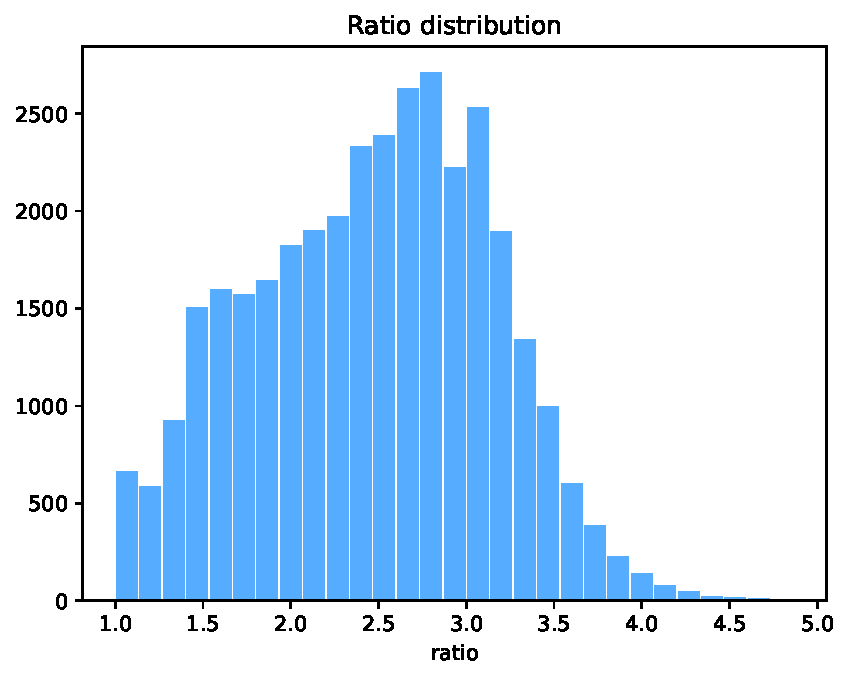
\includegraphics[width=\textwidth]{images/ratio_hist.pdf}
		\end{column}

		\begin{column}{.48\linewidth}
			\justifying{\cBlue{Ratio distribution of UAV-BD.} The ratio ranges from $1.0$ to $5.0$. }
		\end{column}
	\end{columns}
	\note{For better training the CNN-based algorithms, we counted some dataset's data distribution. Including angle distribution, ratio distribution, size distribution.}
\end{frame}

%-=-=-=-=-=-=-=-=-=-=-=-=-=-=-=-=-=-=-=-=-=-=-=-=
%	Dataset Statistics
%-=-=-=-=-=-=-=-=-=-=-=-=-=-=-=-=-=-=-=-=-=-=-=-=
\begin{frame}{Dataset Statistics}

	\begin{columns}
		\begin{column}{.48\linewidth}
			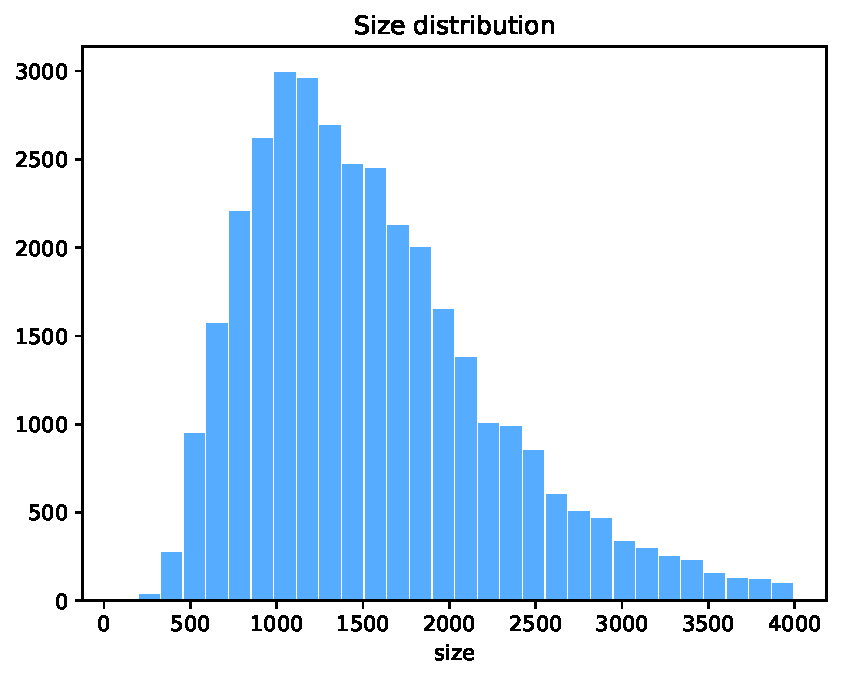
\includegraphics[width=\textwidth]{images/size_hist.pdf}
		\end{column}

		\begin{column}{.48\linewidth}
			\justifying{\cBlue{Size distribution of UAV-BD.} The size ranges from $0$ to $4000$. }
		\end{column}
	\end{columns}
	\note{For better training the CNN-based algorithms, we counted some dataset's data distribution. Including angle distribution, ratio distribution, size distribution.}
\end{frame}



%-=-=-=-=-=-=-=-=-=-=-=-=-=-=-=-=-=-=-=-=-=-=-=-=
%	Dataset Statistics
%-=-=-=-=-=-=-=-=-=-=-=-=-=-=-=-=-=-=-=-=-=-=-=-=
\newcommand*{\vcenteredhbox}[1]{#1}
% \begin{frame}{Dataset Statistics}
% 	\vcenteredhbox{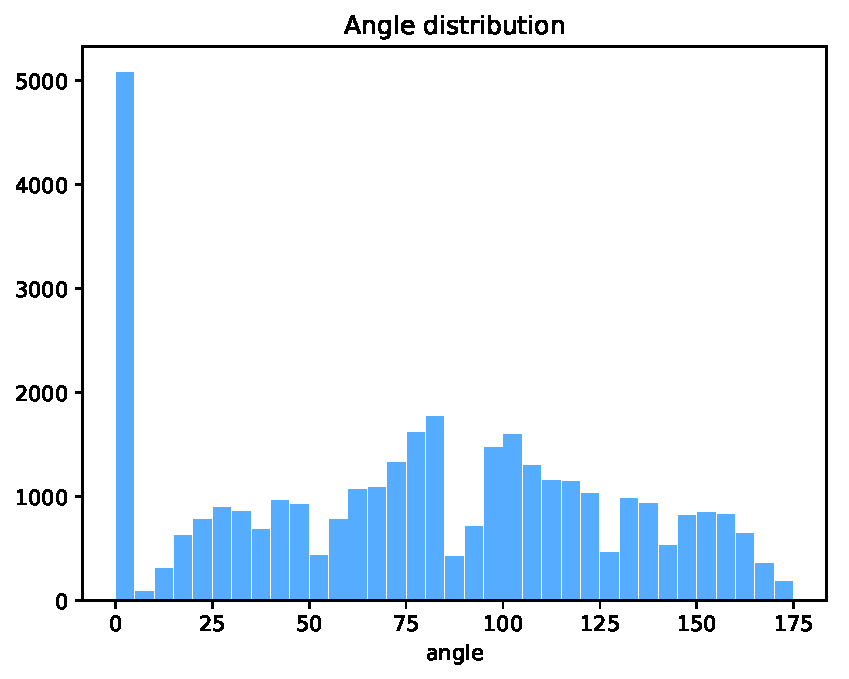
\includegraphics[width=0.33\textwidth]{images/angle_hist.pdf}}
%    	\hfill
% 	\uncover<2->{\vcenteredhbox{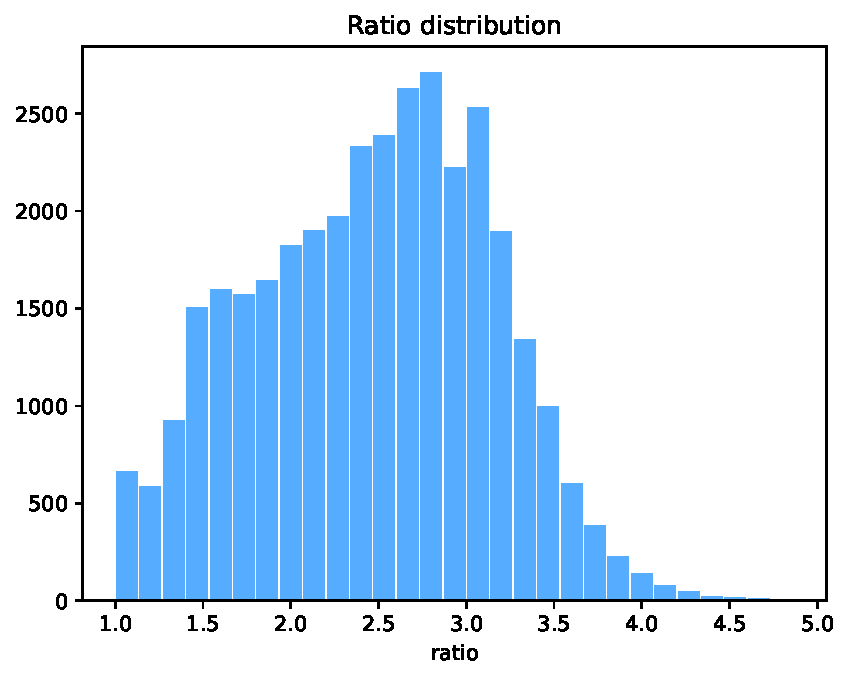
\includegraphics[width=0.33\textwidth]{images/ratio_hist.pdf}}}
% 	\hfill
% 	\uncover<3->{\vcenteredhbox{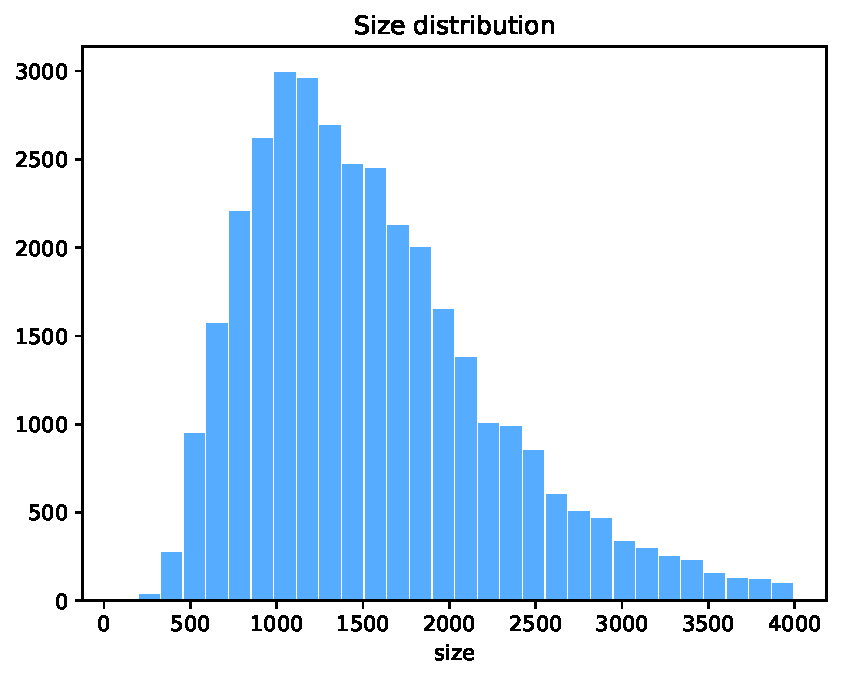
\includegraphics[width=0.33\textwidth]{images/size_hist.pdf}}}
% \end{frame}

%-=-=-=-=-=-=-=-=-=-=-=-=-=-=-=-=-=-=-=-=-=-=-=-=
%	SECTION: Baselines and Methods
%-=-=-=-=-=-=-=-=-=-=-=-=-=-=-=-=-=-=-=-=-=-=-=-=

\section{Baselines and Methods}\label{baselines}

%-=-=-=-=-=-=-=-=-=-=-=-=-=-=-=-=-=-=-=-=-=-=-=-=
%	FRAME: Dataset Split and Baselines
%-=-=-=-=-=-=-=-=-=-=-=-=-=-=-=-=-=-=-=-=-=-=-=-=
\begin{frame}{Dataset Split}
	\justifying{We randomly select \cBlue{$64\%$}, \cBlue{$16\%$} and \cBlue{$20\%$} of the UAV-BD as the \cBlue{training}, \cBlue{validation} and \cBlue{testing} data. So the whole UAV-BD contains $16,258$ images with $22,211$ instances for training, $4,055$ images with $5,624$ instances for validation and $5,081$ images with $6,944$ instances for testing.}
	\note{We randomly select \cBlue{$64\%$}, \cBlue{$16\%$} and \cBlue{$20\%$} of the UAV-BD as the \cBlue{training}, \cBlue{validation} and \cBlue{testing} data. So the whole UAV-BD contains $16,258$ images with $22,211$ instances for training, $4,055$ images with $5,624$ instances for validation and $5,081$ images with $6,944$ instances for testing.}
\end{frame}

%-=-=-=-=-=-=-=-=-=-=-=-=-=-=-=-=-=-=-=-=-=-=-=-=
%	FRAME: Baselines with Horizontal Bounding Boxes
%-=-=-=-=-=-=-=-=-=-=-=-=-=-=-=-=-=-=-=-=-=-=-=-=
\begin{frame}{Baselines with Horizontal Bounding Boxes(HBB)}
	\justifying{We select \cBlue{Faster R-CNN}, \cBlue{SSD}, \cBlue{YOLOv2} as our baseline for horizontal object detection. The experimental results of HBB prediction are shown in figure below.}
	\begin{figure}
		\centering
		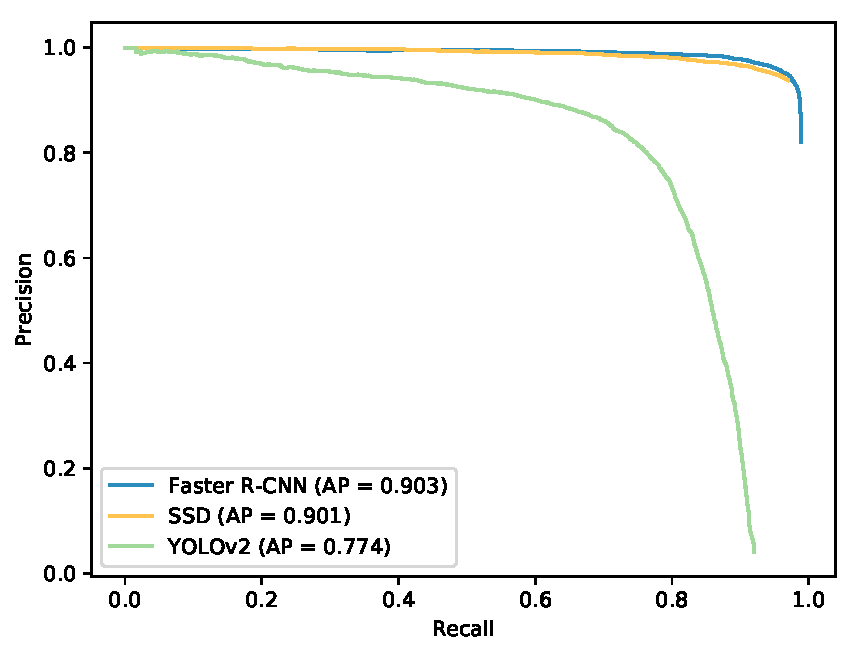
\includegraphics[width=0.6\textwidth]{images/pr_bbox.pdf}
	\end{figure}
	\note{We select \cBlue{Faster R-CNN}, \cBlue{SSD}, \cBlue{YOLOv2} as our baseline for horizontal object detection. The experimental results of HBB prediction are shown in figure below.}
\end{frame}

%-=-=-=-=-=-=-=-=-=-=-=-=-=-=-=-=-=-=-=-=-=-=-=-=
%	FRAME: Baseline with Oriented Bounding Boxes
%-=-=-=-=-=-=-=-=-=-=-=-=-=-=-=-=-=-=-=-=-=-=-=-=
\begin{frame}{Baseline with Oriented Bounding Boxes(OBB)}
	\justifying{\footnotesize{For oriented object detection, wo modify the original \cBlue{Rotation Region Proposal Network(RRPN)} algorithm to predict properly oriented bounding boxes. RRPN's network structure is shown in figure below.}}

	\begin{figure}
		\centering
		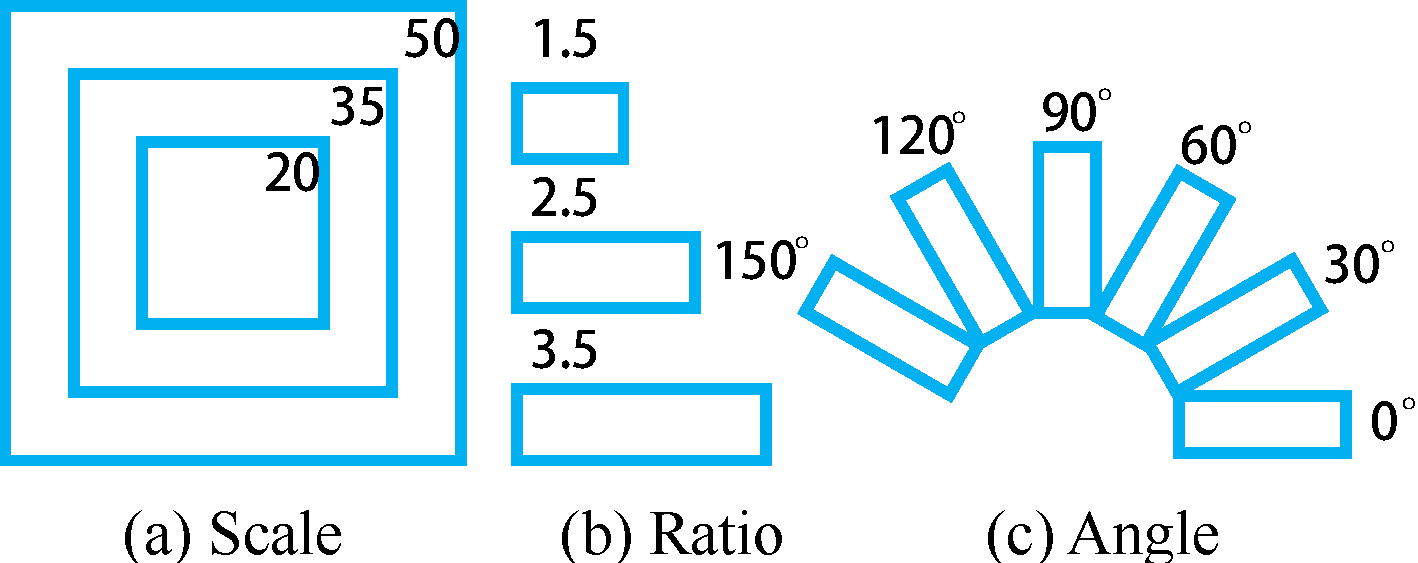
\includegraphics[width=0.4\textwidth]{images/scale_ratio_angle.pdf}
		\par
		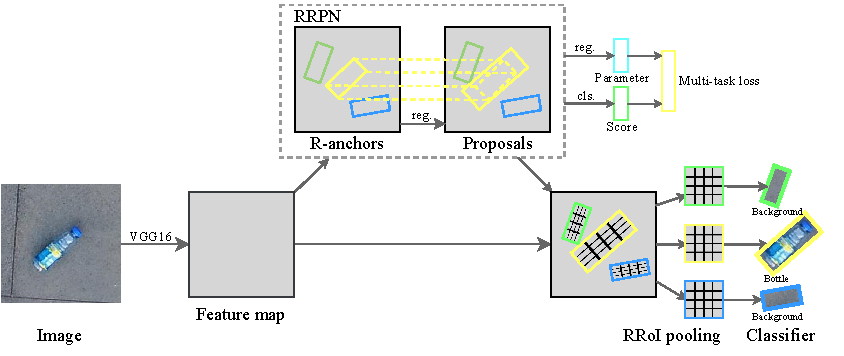
\includegraphics[width=0.85\textwidth]{images/RRPN.pdf}
	\end{figure}
	\note{For oriented object detection, wo modify the original \cBlue{Rotation Region Proposal Network(RRPN)} algorithm to predict properly oriented bounding boxes. RRPN's network structure is shown in figure below. The scale, ratio and angle settings are came from dataset's distribution.}
\end{frame}

%-=-=-=-=-=-=-=-=-=-=-=-=-=-=-=-=-=-=-=-=-=-=-=-=
%	FRAME: Baseline with Oriented Bounding Boxes
%-=-=-=-=-=-=-=-=-=-=-=-=-=-=-=-=-=-=-=-=-=-=-=-=
\begin{frame}{Baseline with Oriented Bounding Boxes(OBB)}
	The experimental results of OBB prediction are shown in figure below.
	\begin{figure}
		\centering
		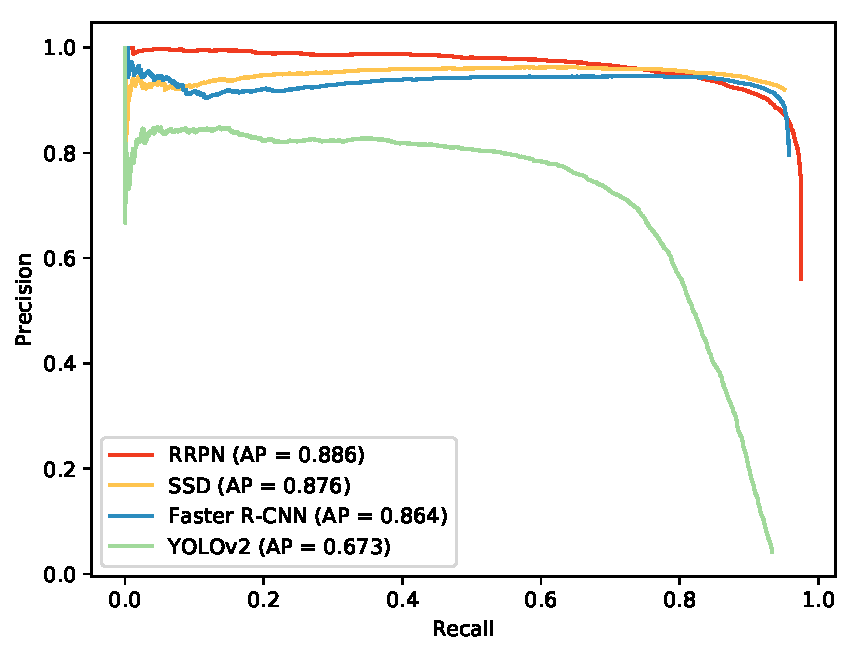
\includegraphics[width=0.6\textwidth]{images/pr_rbbox.pdf}
	\end{figure}
	\note{The experimental results of OBB prediction are shown in figure below.}
\end{frame}

%-=-=-=-=-=-=-=-=-=-=-=-=-=-=-=-=-=-=-=-=-=-=-=-=
%	FRAME: Experimental Analysis
%-=-=-=-=-=-=-=-=-=-=-=-=-=-=-=-=-=-=-=-=-=-=-=-=
\begin{frame}{Experimental Analysis}
	\begin{figure}
		\centering
	 	\includegraphics[width=1.0\textwidth]{images/result.png}
 	\end{figure}
	\note{Bottles detection results in our dataset. As you can see, RRPN's performance is highest.}
\end{frame}

%-=-=-=-=-=-=-=-=-=-=-=-=-=-=-=-=-=-=-=-=-=-=-=-=
%	FRAME: Experimental Analysis
%-=-=-=-=-=-=-=-=-=-=-=-=-=-=-=-=-=-=-=-=-=-=-=-=
\begin{frame}{Some Details}
	\begin{columns}
		\begin{column}{.48\linewidth}
			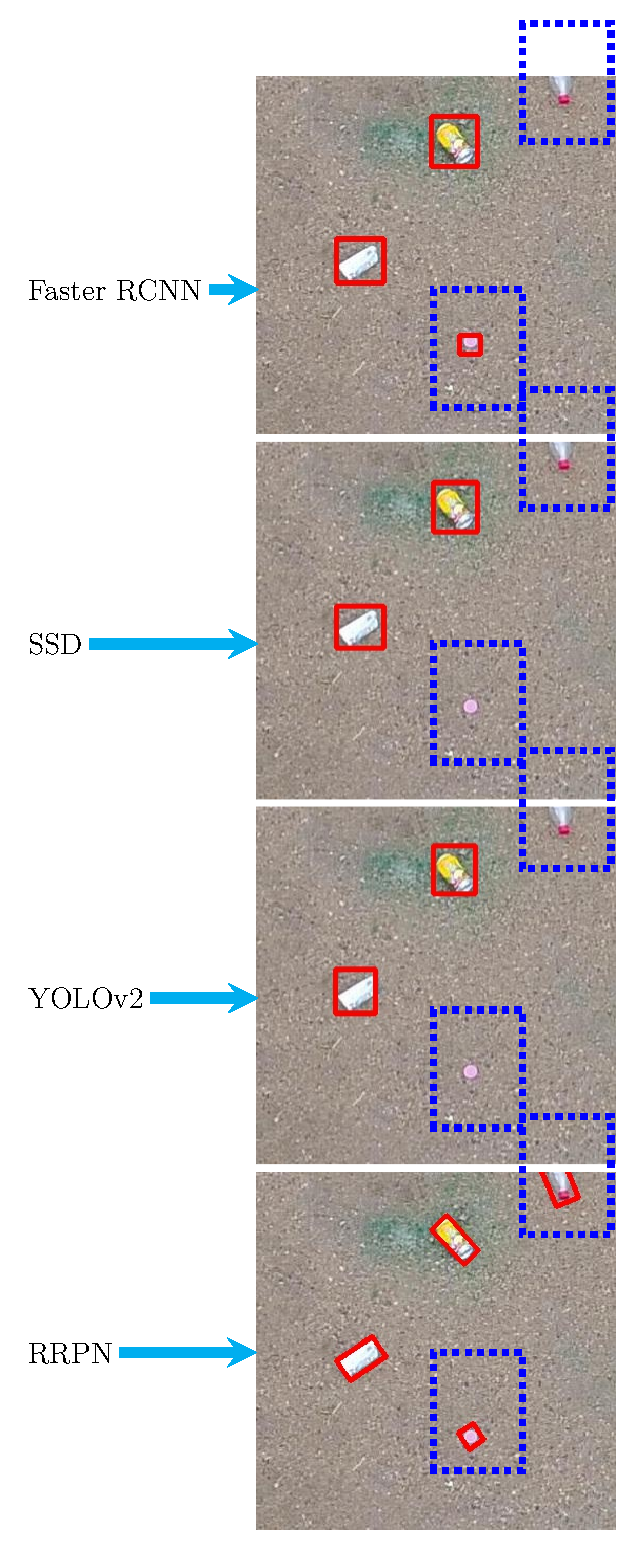
\includegraphics[height=1.0\textheight]{images/results_room1.pdf}
		\end{column}

		\begin{column}{.48\linewidth}
			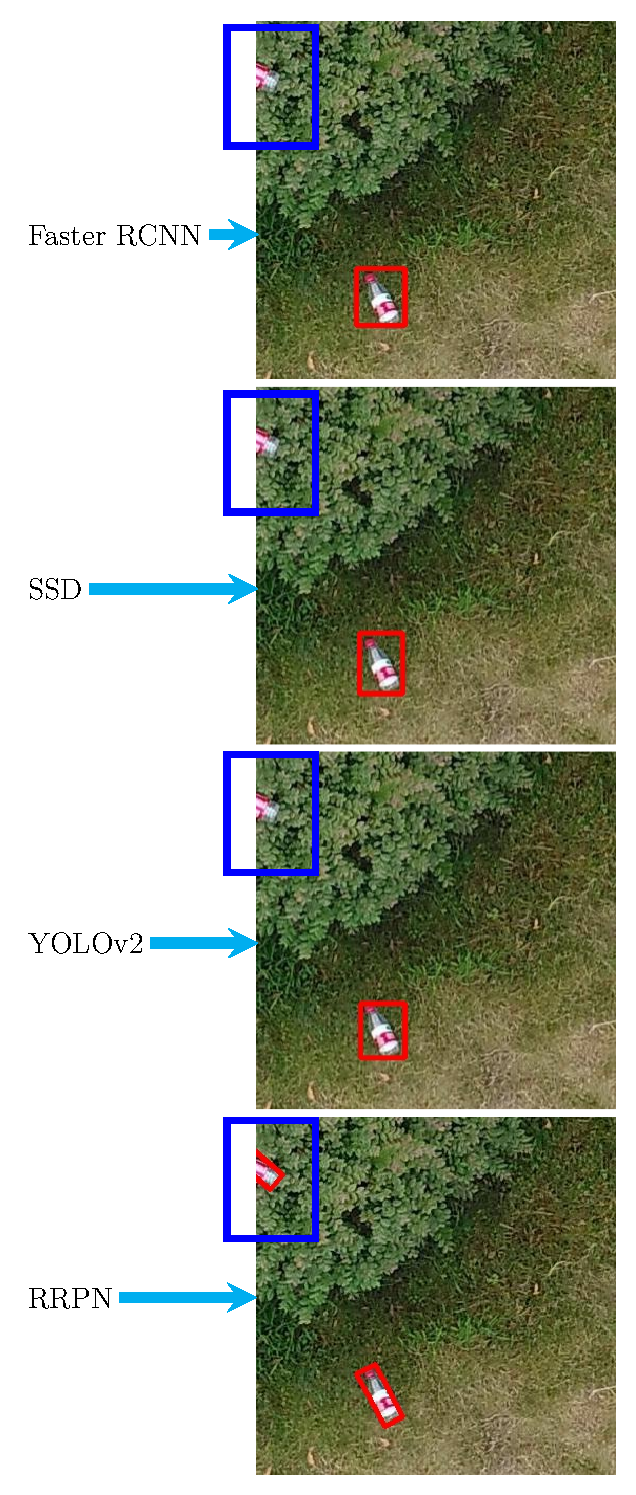
\includegraphics[height=1.0\textheight]{images/results_room2.pdf}
		\end{column}
	\end{columns}

	\note{Bottles detection results in our dataset. As you can see, RRPN's performance is highest.}
\end{frame}

%-=-=-=-=-=-=-=-=-=-=-=-=-=-=-=-=-=-=-=-=-=-=-=-=
%
%	SECTION: Conclusion and Future Work
%
%-=-=-=-=-=-=-=-=-=-=-=-=-=-=-=-=-=-=-=-=-=-=-=-=
\section{Conclusion and Future Work}

%-=-=-=-=-=-=-=-=-=-=-=-=-=-=-=-=-=-=-=-=-=-=-=-=
%	FRAME: Experimental Analysis
%-=-=-=-=-=-=-=-=-=-=-=-=-=-=-=-=-=-=-=-=-=-=-=-=
\begin{frame}{Conclusion and Future Work}
	\cBlue{Contribution}
	\begin{itemize}
		\item<1-> \justifying{Built a large-scale dataset for bottle detection in UAV images named UAV-BD.}
		\item<2-> \justifying{Annotated a huge number of well-distributed bottles with oriented bounding boxes.}
		\item<3-> \justifying{Established a benchmark for bottle detection.}
	\end{itemize}
	\cBlue{Future Work}
	\begin{itemize}
		\item<4-> \justifying{We will focus on locating and recycling bottles in the real-world using UAV.}
	\end{itemize}
	\note{Our contributions including built a large-scale dataset for bottle detection in UAV images named UAV-BD, annotated a huge number of well-distributed bottles with oriented bounding boxes, established a benchmark for bottle detection. In the future, we will focus on locating and recycling bottles in the real-world using UAV.}
\end{frame}

%-=-=-=-=-=-=-=-=-=-=-=-=-=-=-=-=-=-=-=-=-=-=-=-=
%	FRAME: WHERE TO GET DATASET
%-=-=-=-=-=-=-=-=-=-=-=-=-=-=-=-=-=-=-=-=-=-=-=-=

\begin{frame}[c]{Get UAV-Bottle Dataset}
	\vspace{10mm}
	UAV-Bottle Dataset and Development Kit can be downloaded on Google Drive and Github. \\
\vspace{1em}
\begin{center}
	\large{UAV-Bottle Dataset}
	\cBlue{\url{https://jwwangchn.github.io/UAV-BD/}}

	\large{Development Kit}
	\cBlue{\url{https://github.com/jwwangchn/UAV-BD.git}}
	\vspace{1.5em}

	\begin{figure}
		\centerline{
			
\includegraphics[width=0.1\textwidth]{images/GitHub-Mark-120px-plus.png}
			\hspace{1.5cm}
			
\includegraphics[width=0.1\textwidth]{images/Google_Drive_Logo.png}
			}
		% \caption{Hosted on GitHub}
	\end{figure}
	
\end{center}
	\note{You can download our dataset from Google Drive and download develop kit from Github.}
\end{frame}


%-=-=-=-=-=-=-=-=-=-=-=-=-=-=-=-=-=-=-=-=-=-=-=-=
%	FRAME: References
%-=-=-=-=-=-=-=-=-=-=-=-=-=-=-=-=-=-=-=-=-=-=-=-=

\begin{frame}{References}
	\begin{thebibliography}{10}
	\scriptsize
	\beamertemplatearticlebibitems
	\bibitem{dota2018}
	Xia G S, Bai X, Ding J, et al.
	\newblock DOTA: A large-scale dataset for object detection in aerial images
	\newblock IEEE CVPR, 2018

	\beamertemplatearticlebibitems
	\bibitem{RRPN}
	Ma J, Shao W, Ye H, et al.
	\newblock Arbitrary-oriented Scene Text Detection via Rotation Proposals
	\newblock IEEE Transactions on Multimedia, 2018
	
	\beamertemplatearticlebibitems
	\bibitem{FasterRCNN}
	Ren S, He K, Girshick R, et al.
	\newblock Faster R-CNN: Towards Real-time Object Detection with Region Proposal Networks
	\newblock Advances in Neural Information Processing Systems, 2015
	
	\beamertemplatearticlebibitems
	\bibitem{SSD}
	Liu W, Anguelov D, Erhan D, et al.
	\newblock SSD: Single Shot Multibox Detector
	\newblock ECCV, 2016
	
	\beamertemplatearticlebibitems
	\bibitem{YOLO}
	Redmon J, Farhadi A.
	\newblock YOLO9000: Better, Faster, Stronger
	\newblock IEEE CVPR, 2017

  \end{thebibliography}
  \note{There are some references.}
\end{frame}

%-=-=-=-=-=-=-=-=-=-=-=-=-=-=-=-=-=-=-=-=-=-=-=-=
%	FRAME:
%-=-=-=-=-=-=-=-=-=-=-=-=-=-=-=-=-=-=-=-=-=-=-=-=
\begingroup
\setbeamercolor{background canvas}{bg=\cnDarkGrey}
\begin{frame}[plain]
\vspace{1.4cm}
\centering{\cGrey{\Huge{Thanks!}}}

\end{frame}
\endgroup

\end{document}
